\chapter{Trash in Culture and Theory}





% FROM Uncle Fernando’s Garbage Triptych, http://alphabet-city.org/issues/trash/articles/uncle-fernando-s-garbage-triptych, http://priscilauppal.ca/books/alphabet-city/
\epigraph{Anger is nothing compared to garbage:\\ Garbage eats anger for breakfast.\\ It eats all of us in the end.}{\hfill---Priscilla Uppal, \quotes{Uncle Fernando’s Garbage Triptych}}





%
%
In this chapter trash and the practice of transforming trash is examined in theoretical and conceptual aspect. Theoretical foundations of trash (Rubbish Theory) are discussed. Beyond common perception and dictionary meaning of trash alternative or different approaches are examined with help of ideas of philosophers (Zizek). Focused on the type of trash (disposable, single-use trash) and questioned the behavioural pattern that generates mountains of trash with these disposable trash. Further it is mentioned how artist are approached these notions? and how their work viewed as their offered window or framework.





%
%
\section{Throw away culture}
[What is questioned in this section?] Firstly we need to ask what is the source of trash. How is it generated? Secondly what are the behaviors behind the producing trash?





%
%
[Disposable items.] \comment{Disposable: made to be used once or only a few times. Made to be thrown away after one use or several uses. Not permanent or durable. Not designed to reuse again and again. For examples packages of bevarages, paper cups etc. They are used very short-time. Their lifetime can be measured in minutes in terms of usage. I have never seen such person that uses own paper cup again and again. However their usage durations are very short, they continue to exist in the nature.} \todo{transition gerekli.} \paraphrase{The strange think about many products that are produced these days is that they are not made to last for a long time. Importantly the term throw away society has a slightly negative connotation, or meaning. When you describe a society as a throw away society, you are probably critising that behaviours or showing your disapproval. \todo{ref.}} 


\paraphrase{being wasteful in the ways we live is encouraged, expected and in many instances impossible to avoid (Hawkins 2006: x)}

Disposable items are first introduced X and their usage accelerated after Y. There are Z factors that give rise to usage of single-use ites excessively \todo{Bu cümleyi doğru düzgün kurmak gerekli.}.

% Reference from Identity, mobility and the throwaway society
[The term throwaway culture] Life magazine first introduced the term "throw-away" mentioning that behavioral pattern of society \todo{life magazine tekrar bak.}. \comment{Scholars argue that contemporary societies are throwaway societies (Barr, 2004; Cooper, 2003, 2005; Cooper and Mayers, 2000; Strasser, 1999, cf. O’Brien, 1999; Hawkins and Muecke, 2003) \todo{ref required.}.} The term is actually a criticism of over consumption of short-live disposable objects. \comment{The term overconsumption refers to a way of living in which the lifestyle patterns of human beings lead to an accelerated expenditure of natural resources.}

\paraphrase{Life magazine fashionably heralded the advent of the "throwaway society" in 1955. 1971 daniel ingersoll reporting on his findings in the journal man in the notheast, "the industrial revolution ... was supplying the customer with hundreds of disposable containers and materials bt the end of the nineteenth century. the estimated 25.000 cubic yards of fill deposited in the upper portion of puddle dock show that the age of the throw away world began not in the twentieth century but during the nineteenth."} \todo{ref. Hangi kaynaktan?}

% Reference from Identity, mobility and the throwaway society
[Counter-argument] Even if conducted a qualitative research people are really do not throw away their things. \paraphrase{The research did not include the leftovers and detritus of food consumption packaging, bottles, and food waste, for example and neither was it concerned with another major category contributor to the volume of household waste, those `disposable' goods that are the primary means to maintaining bodily hygiene and cleanliness (Shove, 2003)}. They analyzed the things like television, furniture and toys like that.

[Factors.] \comment{Not only one factor, technological advacements can be one of them. These items with the help of industrialization can be produced easily. Mass production. Disposable items are reduces the labour and human resources as compared to the traditional ways (Consider napkin vs wipes, glass vs paper cup). Another point is that they are more affordable in terms of supply chain and cost. In other words you can put new one easily. Therefore there is no need to save the old one. Last but not least increasing attention of hygine is contributed to the extension of disposables in the market highly.} \paraphrase{The commodities of food and drink must be safe, sterile and private.} \todo{ref. ontology of trash}

\paraphrase{Taken to its obsessive extreme, the germ theory proscribes companionship. The Latin root for this word, cum pani, literally means to share bread. But insofar as each eater harbors untold numbers of hazardous germs, it is safest to keep one’s food strictly to one’s self. Safety in a world of bacteria implies isolation. Packaging successfully isolates both food and consumer within a structure of sterile control. In essence, it encloses the commons. Susan Strasser narrates part of the history of this enclosure through the career of the disposable drinking cup, which appeared in the early years of the twentieth century. \todo{ref. ontology of trash}}

\begin{quote}
While the sanitary advantages of toilet paper might have been obvious, those of the paper cup required a belief in germs. The widespread use of paper cups was a direct result of a public health crusade educating people about the invisible organisms spread by the common drinking cups once standard in public places, especially trains and railroad stations. Manufacturers of paper cups teamed up with public health authorities to campaign for federal and state regulations banning common drinking cups from use in interstate traffic. Succeeding in 1912, they competed for the business of the railroads and train stations\ldots
Disposable paper cups met significant resistance. Most public places offered them in coin-operated dispensers, and some people were not willing to pay for what had once been free. Respectable travellers carried their own cups, available in metal and celluloid in a variety of collapsable and folding designs. Others reused paper cups from the trash or drank out of the public tanks, putting their lips to the faucet or using the cover of the tank as a cup. Some people protested against the vending machines: soldiers smashed paper cup dispensers in Washington’s Union Station during President Wilson’s inauguration in 1913. And some public places installed drinking fountains instead of paper cups dispensers, although at first these, too, were attacked as unsanitary because people could touch the nozzle with their lips.
\end{quote}

[Dark side.] Usage of disposable items in the society is very widespread. For same cases it is inevitable. Beyond the advantages of disposable items there are side of effects of consuming them excessively. They result in mountains of garbage.

\comment{Handling of this mountains of garbage is another topic. It is not the topic of this thesis. It is not debated that usage of disposals are supported or not supported. It might be subject of another thesis. What is important here the results of it and the reflection of the artist.} \comment{Buna karşı geliştirilen bir refleks olduğu için bu kısma giriyorum. Aynı zamanda ben de bu ürünü kullanıyorum. Konuyu o yüzden farkl açılarından anlamak gerekli. \todo{Ama benim konuya nasıl yaklaştığım biraz belirsiz.}}

[Art] There are some artists whose works are related with the pheomena expressed above. (Some of the works of artist can be examined in this pheomena.)


% ARTWORK
% Portraits of Global Mass culture
\begin{figure}[h!]
\centering
\begin{subfigure}{.47\textwidth}
  \centering
  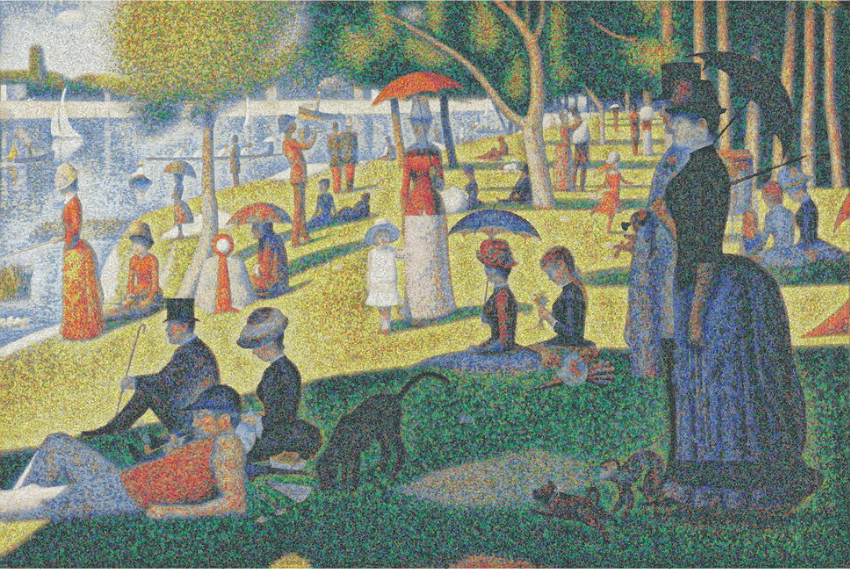
\includegraphics[width=\linewidth]{graphics/ChrisJordan_Numbers_OriginalView.jpg}
  \caption{Original view}
  \label{fig:ChrisJordan_Numbers_CloseView}
\end{subfigure}
\hfill
\begin{subfigure}{.47\textwidth}
  \centering
  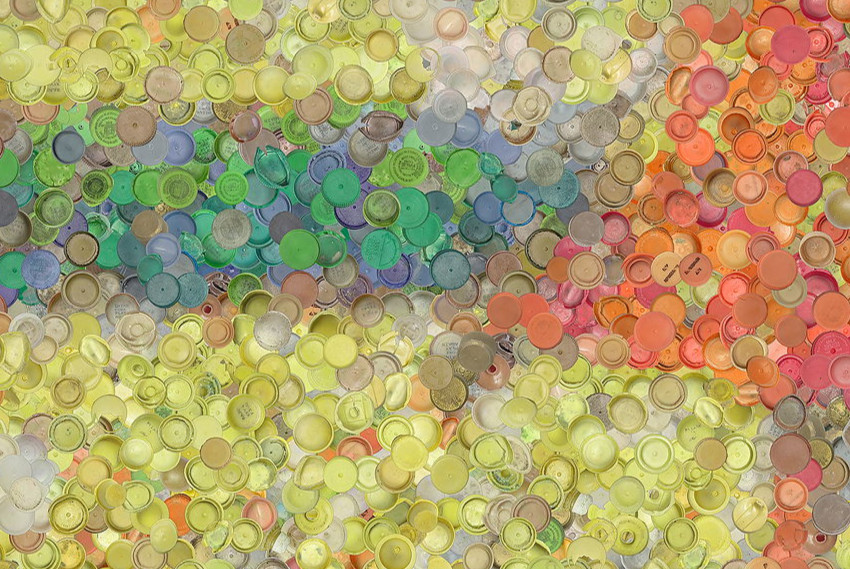
\includegraphics[width=\linewidth]{graphics/ChrisJordan_Numbers_CloseView.jpg}
  \caption{Close view}
  \label{fig:ChrisJordan_Numbers_OriginalView}
\end{subfigure}
\caption{Caps Seurat, 2011 60x90" in one panel, and 88x132" in 3 panels}
\label{fig:ChrisJordan_Numbers_CapsSeurat}
\end{figure}

Chris Jordan creates digital photographic series that turns numbers to visuals. Provide different way to understand the statistics and the missed reality of consumerism. Creates gigantic prints to express numbers in a visual manner. Draws attention the the global consumerism. reveals the reality that is hard to understand. Because it is spread to the community and time.

\paraphrase{Portraits of Global Mass culture from Chris Jordan. Depicts 400,000 plastic bottle caps, equal to the average number of plastic bottles consumed in the United States every minute. In Running the Numbers, photographer Chris Jordan attempts to convey the vastness of modern consumption by breaking down annual statistics into more graspable quantities depicted by clever visualizations made of individual objects or groups of objects that he photographs. “There’s a disconnect that happens when we assume we know what we’re talking about when we talk about hundreds of millions of plastic bottles,” Jordan says. “I’m trying to translate these numbers from the deadening language of statistics into a visual language that allows some kind of comprehension.” Many of Jordan's works are created from photographs of garbage and mass consumption Jordan uses everyday commonalities such as a plastic cup and defines the blind unawareness involved in American consumerism. His work, while often unsettling, is a bold message about unconscious behaviors in our everyday lives, leaving it to the viewer to draw conclusions about the inevitable consequences which will arise from our habits. He recreates the most remarkable artworks with combining bits of trashes as a mosaic. Here he draw attention to the our consumerism and express them numbers that are very big to understand. All the material that we have is trash to create this pictures.}

[CRITICS] Visuals of Chris jordan are like modern versions of mosaics. In the age of consumption the most easily accessible matariel is trash. Trash has different colors and sizes and shapes. Therefore it is a perfect material to build sculptures from them. There is a great diversity of trashes and offers new alternatives.

Not every people throw away disposible objects, some of them save them and use for their own purposes. 


% ARTWORK
% TEA BAGS
% FROM https://instagram.com/silvirub/, http://www.rubysilvious.com/363-days-of-tea
\begin{figure}[h!]
  \centering
  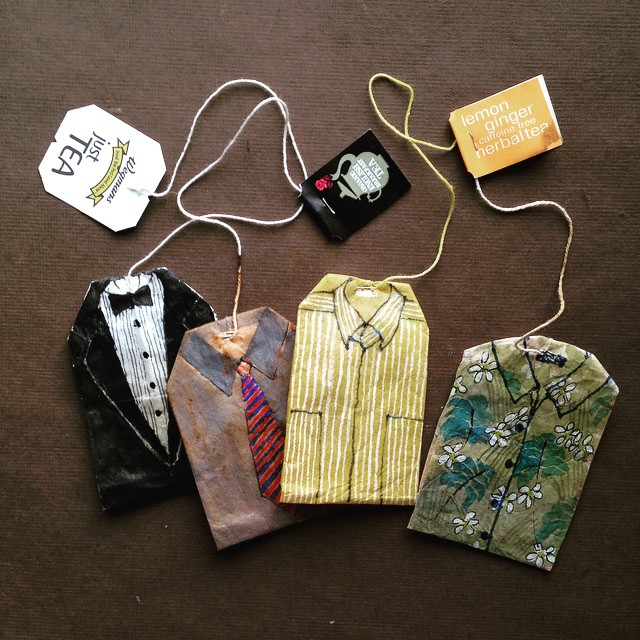
\includegraphics[height=6cm]{graphics/rubysilvious-teabag-Day169.jpg}
  \caption{Ruby Silvious, Day 169, 363 Days of Tea, 2015, Mixed media on upcycled paper tea bags, Dimensions variable}
  \label{fig:RubySilvious_TeaBag}
\end{figure}
  
\paraphrase{Visual artist and graphic designer Ruby Silvious embarked on a quirky, personal experiment, set to last for 363 days. She decided to repurpose soggy and stained tea bags as unconventional, blank canvases, just waiting to be filled with her artistic expression. The project, entitled 363 Days of Tea, allows Silvious to challenge herself by transforming the recycled material with her intricate illustrations—the artist draws, paints, and forms collages on the salvaged tea bags. This project serves as Silvious’ daily journal, allowing her to record her thoughts and feelings by creating wonderful moody and whimsical designs on little teabag papers. Every day she creates a new piece that reflects her impressions in that moment. endeavour of re-purposing recycled and found materials.} \todo{cite website}

[CRITICS] This work is for fathers day. Works of Silvious catch the important moments of days and can be as a diary (or a record of that moment and day). Trashes trasnformed to diaries. Trash is every where, already at hand.


% ARTWORK
% COFFEE CUP
% FROM http://www.gwynethleech.com/
\begin{figure}[h!]
\centering
\begin{subfigure}{.47\textwidth}
  \centering
  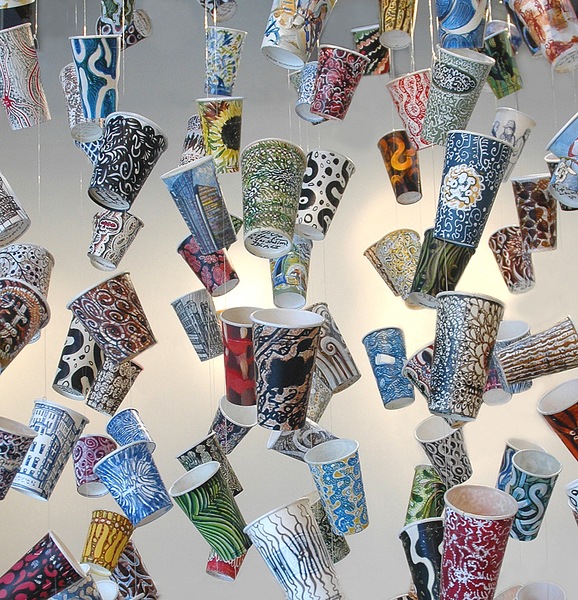
\includegraphics[width=\linewidth]{graphics/Gwyneth-Leech-cup5.jpg}
  \caption{Installation view}
  \label{fig:GwynethLeech_Installation}
\end{subfigure}
\hfill
\begin{subfigure}{.47\textwidth}
  \centering
  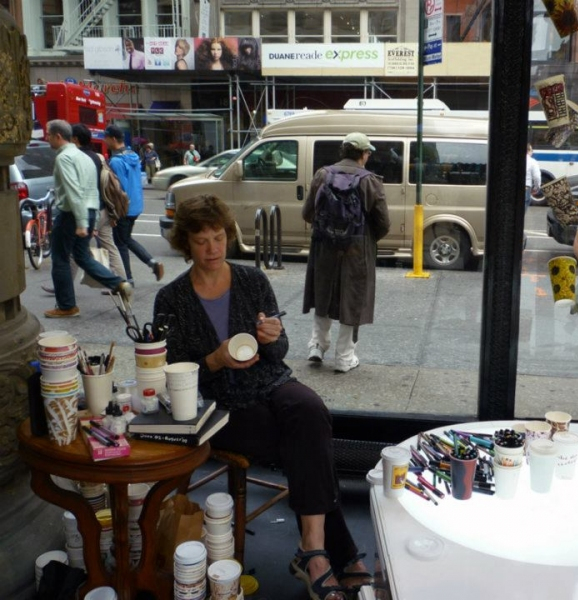
\includegraphics[width=\linewidth]{graphics/Gwyneth-Leech-cup3.jpg}
  \caption{Painting in the public}
  \label{fig:GwynethLeech_Public}
\end{subfigure}
\caption{Gwyneth Leech, 365 A Year in Cups, 2013, Mixed media on upcycled paper coffee cups, Dimensions variable}
\label{fig:GwynethLeech_CoffeeCups}
\end{figure}

\paraphrase{I began to save all of my coffee cups to use as "canvases" for making art. Transforms coffee cups that are no longer trash but a vehicle for art, ideas, conversation and memories of a social moment upcycled from the detritus of our throw-away caffeine culture. I like my coffee or tea in a paper take-out cup. Even better than the contents, I like the used cup as a surface on which to draw and paint. And on the bottom of each one, I write the date, location, occasion and beverage consumed so that every hand-made cup artwork becomes the record of a social moment. Each cup representing a daily caffeine break. The installation makes visible largely unconscious patterns of consumption; this is what one simple take-away purchase looks like over the course of three years, this is what would usually be thrown away. It can be seen as a measure of time gone by, of money spent, of space to be taken up in a landfill. But as I upcycle each used cup into an artwork, it becomes the measure of other things as well: an artist's regular habit of generating new ideas, a diary of time spent with friends and colleagues, and the cumulative positive effect of doing something small and manageable every day. There are different versions of it. paintings on paper coffee cups displayed as installation in public window spaces. She publicly draw their cups (the cup art window installation and public drawing project were on view repeated showed at many places and date. During public drawing projects she draw with other people. and so. Buying a beverage is a daily event for Leech (and also many people. These coffee shops all around the world. As she drinks her coffee in the public, she also publicly transform its cup.} \todo{cite her website}

[CRITICS] inside of glass window. public space. publicly drawing, as she drinks her coffee publicly, also paints them publicly. 





%
%
\todo{transition needed.} [TRASH and POTRAIT OF PEOPLE] Trash tells about societies and also reveals personal aspects of peoples life. What people consume is actually tells many things about them \todo{Bununla ilgili bir sürü referans var, onları buraya ekle.}. As scholars mentioned that throughout the discards of someone else many thing can be understand. They are end product of our activities and it can be traced through the discard and garbage. 






%
%
[GARBOLOGY] Garbology is a study of waste as a social science. Applying methodologies of archeology to the human debris. 

\paraphrase{Weberman infamously used techniques of what he deemed garbology to uncover what he saw as the essential nature of people. He once said, perhaps indirectly referencing Jean Brillat-Savarin’s quote about food, \quotes{You are what you throw away.}" \cite{lukas2012garbage}}

% Garbology, from Encyclopedia, Abhijit Roy
\paraphrase{The field of garbology involves the study of refuse and waste. It enables researchers to document information on the nature and changing patterns of modern refuse, hence assisting in the study of contemporary human society or culture. According to the Oxford English Dictionary, the term was first used by waste collectors in the 1960s. Weberman popularized the term in describing his study of Bob Dylan’s garbage in 1970. It was pioneered as an academic discipline by William Rathje at the University of Arizona in 1973.}\todo{ref.}

\paraphrase{the work of archaeologists such as William Rathje and Cullen Murphy has offered significant insights into the relationship between archaeological artefacts and garbage, exploring the function of trash as a resource for understanding cultural and social practice. At the same time, thinkers such as Zygmunt Bauman and Giorgio Agamben have shed light on the fate of   the human being as a wasted or discarded element in discourses of socio-political hygiene. (from Trash Culture)}

\todo{transition needed.} With the help above understanding of trash, what can we see the work of arts. For examples tracey emin.

\begin{figure}[h!]
  \centering
  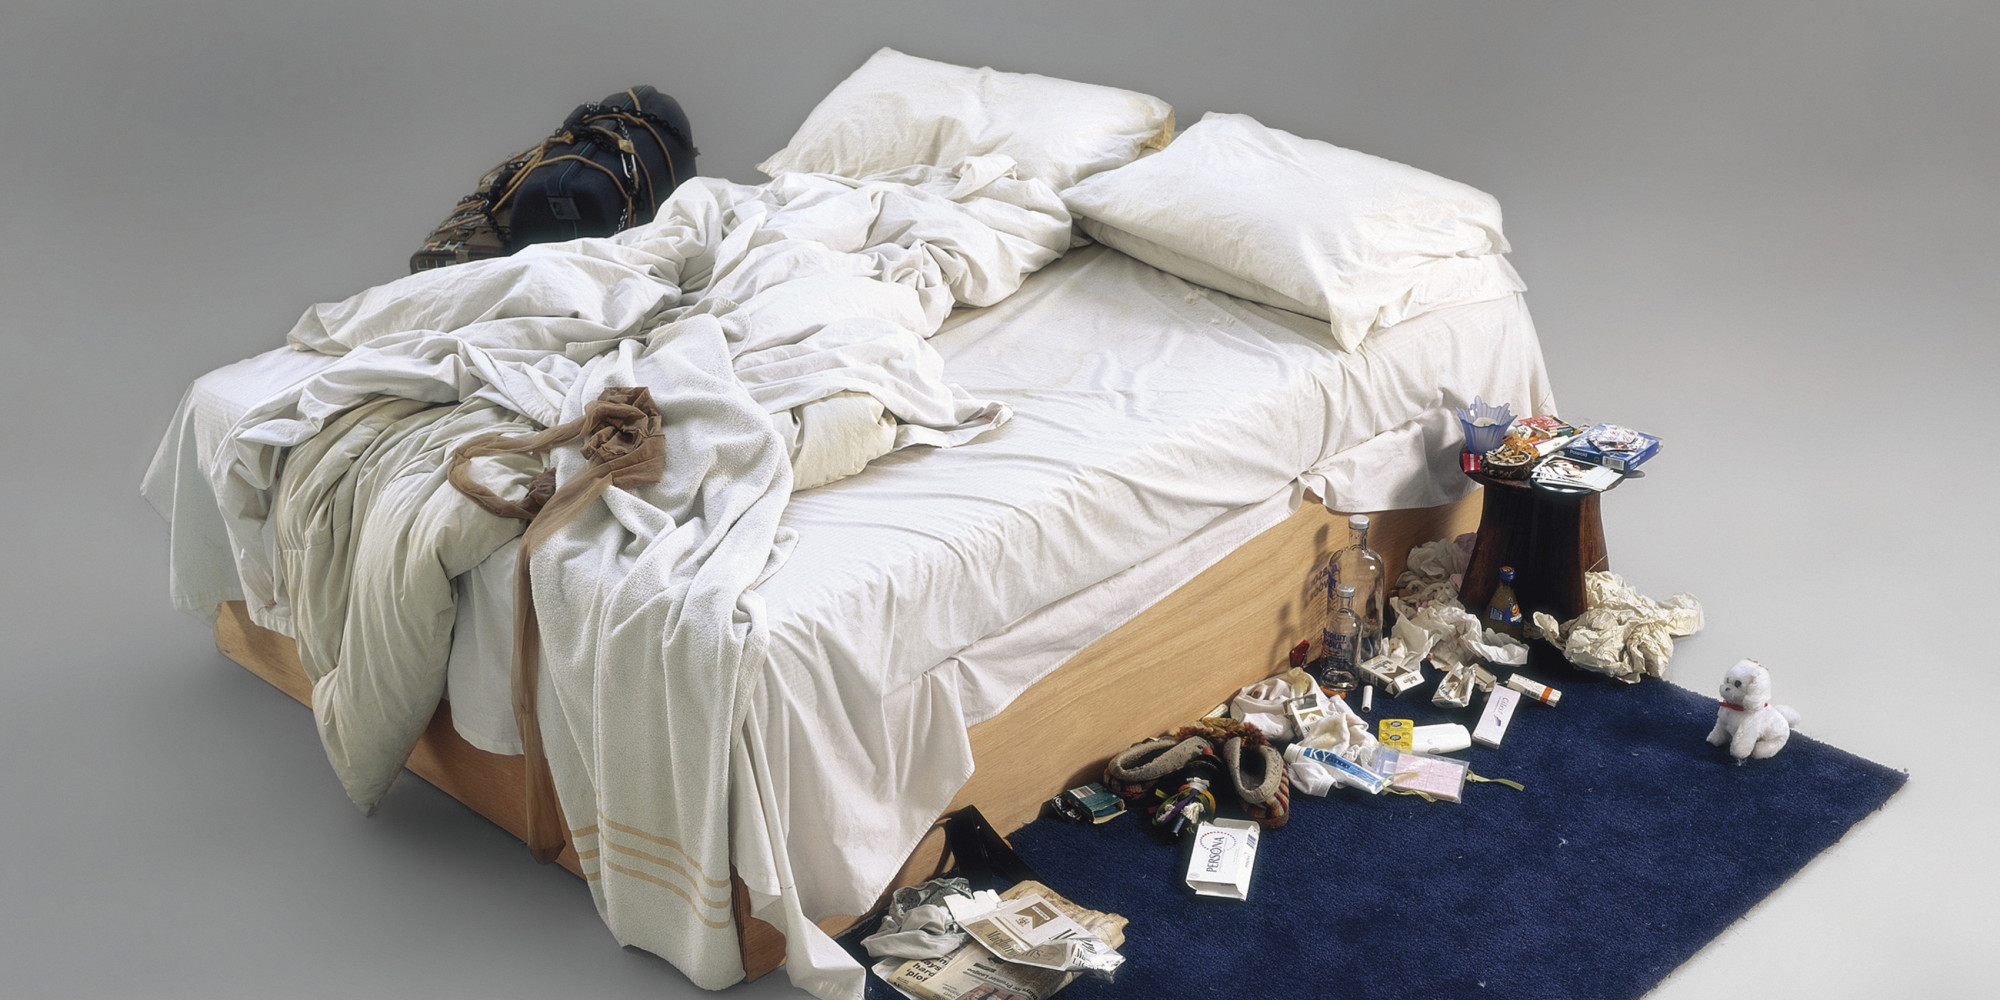
\includegraphics[height=6cm]{graphics/tracey-emin-my-bed.jpg}
  \caption{Tracey Emin, My Bed, 1998}
  \label{fig:TraceyEmin_MyBed}
\end{figure}

\paraphrase{Tracey Emin puts her private life to the public. The work, which Emin now describes as a portrait of a young woman. It is a time capsule. The cigarettes that litter the floor will one day no longer exist; neither will the newspapers. Around her there are pieces of junks speared all over the room. We can understand from her junk what type of life her has. We enter the world of artist through the her trashes.} \todo{Hastalık dönemi... Sanattaki yerine bakmak gerekli.}





%
%
\section{Zizek's Approach to Rubbish}
[Transition, introduction] 
\todo{Adam bir transition bulmalı buraya.} Last decades increasing attention the the ecology and rubbish. This section is related with the increasing interest on ecology. Global warming is one of them, plastic pollution on the oceans also is part of it. These types of news and talks increasingly find a place on media more and more. Zizek comments on ecology and trash.

In documentary film, Examined-life, Zizek, dressed as a sanitation man, talks about ecology in the middle of a garbage dump in London. His part starts with these sentence: \quote{This [garbage dump] is where we should start feeling at home}. 

Draws attention to notion of even if trash disappears from our world but not world. It seems as though the thrown out garbage disappears from our world. However, it disappears only from the world of illusions, but still exists in reality. \comment{Getting rid of it is not action of production. It is action of ignorance. It still waits us at somewhere else or the next generations will have to cope with it. Maybe (as Zizek suggest) the first thing to do is accept the trash.}

He asserts his claim at first and go through explaining how ecology turns to ideology and mentions wrong perception about the ecology. He thinks that the way of approaching ecology is problematic, because accepting that nature as a balanced harmonious thing. He claims that it is ideological in the sense that wrong thinking important problems. Nature contains unimaginable catastrophes. Consider distinction of animals and creation of oil. People profit from the balance of the nature but it is created from a series of catastrophes. He asserts that ecology will slowly turn to religion that \quotes{is a kind of an unquestionable highest authority.} Ideology of ecology warns us like, \quotes{Don't do that. It would be too much.} its voice is like \quotes{Don't mess with D.N.A. Don't mess with nature. Don't do it} etc. He suggests that people must more alienated from the nature. They must find poetry and spirituality in the dimension of trash. That's the true love of world. Love is not about idealization. Therefore he thinks that garbage dump is a place that people should accept it as a home.

\quotes{According to Zizek, modern understanding of ecology is the real false consciousness, connected with mystification of real problems. Postmodern mysticism arises when disasters begin to be rationalized, interpreted in strict logic terms of cause-effect relations. Such interpretation makes life easier. However, nature is not an absolute balance and total harmony (this aspect of Zizek’s thought makes him akin to classical conservatives). Nature is a series of unthinkable disasters. Zizek believes that ecology is transforming into a new western conservative ideology: “One should not play games with nature! Do not touch DNA! Do not develop new medicines! Do not invent new technologies!” How one should react to these reproaches? Zizek’s recipe is to reinforce alienation from nature, to become more artificial.} \cite{vafin2012zizek}

\paraphrase{His basic argument is that the modern eco movement is a conservative ideology. It says don't do X from an authoritarian high ground and it idolizes and mystifies ecology. Basically he says the eco movement has it's head in the clouds. If it loved the environment it would recognize the rubbish we create and the chaotic nature of ecological change and try to further divorce itself from that process(nature) and try to turn the whole thing into art.}

Some of his ideas can be summarized as follows:
\begin{itemize}
\item Our relation to our filth follows an “out of sight, out of mind” principle, but trash doesn’t disappear.
\item Ideology addresses real problems but mystifies them.
\item We search for meaning when a horrible event happens to make it easier to accept.
\item The ideology of ecology is that world is in the best possible state and that humans disturb nature.
\item Nature is not an organism in balance that humans exploit, but rather a series of great catastrophes.
\item Ecology is becoming more like religion with dogmas.
\item Even if we learn the potential catastrophes of nature, we ignore them as long as they don’t manifest near us.
\item The solution is not to worry about saving nature, but to figure out how to survive without it by becoming more artificial.
\item Learn to love our trash as a part of ecology.
\end{itemize}

Some artists turned to trash into site-specific sculptures that are more than trash heap after their intervantion. Not discarding but bracing our attitudes turned them to a something that worth it to watch and think about it. (Converting what we create harmonious with the existing system. Because it is not possible to think that nature will live harmoniously what we created. The more likely idea will be we will live harmoniously with what we create.) Turning trash to things that can be lived together \todo{Buraya sanat işi gelebilir, özellikle kamusal alana yapılan çöten heykel işleri gibi.}.

\todo{needs a discussion.}

[Summary.] \comment{Sürekli çöpü kendimizden uzak tutmaya çalışırken aslında zizek bize bunun tam da tersini yapmamızı bize öneriyor. Bu adam aslında insanlar doğaya zarar vermiyorlar demiyor. Onun dediği aslında yanlış sebep sonuç ilişkileri kurduğumuz üzerinden gidiyor. Çöpü tekrar ele aldığımızda ise yep yeni şeyler keşfedeğiz. Yeni alternatifler oluşacak. Aslında yeni bir dünya kurgulanacak. Çöp nasıl dönüştürülecekse, çöp de insanları dönüştürecek.}

Transforming trash is not related with ecological perspective. We are not trying to save the planet earth or mother nature. Beyond ecological concerns we are trying to find ways to live our trash. 

Zizek mentions that ecology is something wrong point to approach trash. Shows the problematic understanding of garbage. Suggest another thing, and point out the need for the new approach. Beyond the ecological problem there are different sides of it. Different readings can be added to the topic. Adding spirituality and new aesthetics dimension to the topic. 

Idealization of nature is problematic. Loving nature is loving trash. Live with trash. Do not see it as trash actually. Then the question is How to love trash? How to live with trash? Think beyond the common perception. Do not think it as abject, disgust. Can living with our trash enrich (our perceptions, abilities)? How not to see them as trash and useless? Can it be possible with art?

\todo{Çöp evler buraya gelebilir belki, çöpleriyle birlikte yaşayanlar?}





%
%
\section{Rubbish Theory}

\comment{Çöpün hep çöp gibi kalmadığı ve farklı bakış açıları olabileceğini gördük. Bu hareketlilik ve farklılık ise bir teorik çerçeveye oturulmuş, hadi ona baklım şimdi. Zaten bu hayatta çöp her zaman karşımıza çöp olarak çıkmıyor.}

In this thesis transformation of trash is claimed and this theory provides a framework for this transformation. 

\paraphrase{Michael Thompson’s 1979 study Rubbish Theory elaborated an understanding of rubbish as part of a flexible and shifting system of value construction, underlying notions of innovation, creativity and social status \todo{ref. from Trash Culture}.}

\paraphrase{The potential of the discarded thing also relies on its status as a thing approaching a \quotes{zero point} of value. In other words, it has reached a point in transition between the world of the functioning, the useful and visible, and the realm of the invisible, the non-functioning and empty. As Michael Thompson’s Rubbish Theory  suggests, at its nadir in a cycle of consumption and production, rubbish is both ready for disappearance and yet ripe for reinvestment, reinterpretation or revaluing \todo{ref. from Trash Culture}.}

\paraphrase{Objects have a lifetime and they don't remain same through that lifetime. Their value, usage, location change over time. During its lifetime objects may circulate different markets and values systems like economical value, social value, aesthetic value etc. Especially this cycle has picked up speed with the advent of consumer culture, our most recent technological gadgets becoming obsolete within 3 years. Objects function and value are transformed by relocation and revaluation of objects from one place to the other or one discipline to another. This flow(transition) and transformation theorized with Rubbish Theory by Thompson \cite{thompson1979rubbish}. Thompson looks at the creation and destruction of value in man-made objects, cultural artifacts, and ideas. He notes how an object’s economic and/or cultural value diminishes over time rendering the objects worthless or redundant. The theory looks at how some of these objects then regain value, such as antiques or historic homes. It claims that there are three types of objects; transient (normal state, decreasing value, circulating), durable (permanent, increasing value, removed from circulation) and rubbish(zero value, will be destroyed or reinvested for economic and social value). The transition from transient to durable is only possible firstly transient to rubbish and later rubbish to durable. Further, there is a common idea/argument/motto that is "trash to treasure" among artists who use trash as a medium. Rubbish theory presents a conceptual approach to this argument.}

Although Thompson is quite successful categorizing states of objects throughout their lifetime, claimed transitions between states in the theory have some problems. Thompson label some transitions as possible and the others as impossible. \quotes{He allows goods only to move from a transient to become rubbish, and from rubbish they can either be destroyed or become durable. Movement in the other direction, from durable to either transient or rubbish, is not allowed in this system} \cite{meadow2011relocation}. Further, he does not allow move from transient to durable. However, Duchamp's fountain breaks this rule. Because urine used as a fountain is still functional and have a place in the market. In another word, it is not rubbish. This urine with the intervention of Duchamp turned to be an artwork. It is one of the most influential piece of modern art and one of the best examples of ready-made. After Duchamp's intervention to the urine, it becomes a durable object placed in a museum \todo{Fontain's importance in the history of art} \todo{what happens when we look at from the eyes of rubbish theory}.

\paraphrase{In rubbish theory beyond the objects states how it happens transition of objects in practice is missing and Parsons fills this gap by claiming that transition from rubbish to durable are possible with finding objects, displaying objects, re-using objects \cite{parsons2008thompsons}.} 

\paraphrase{Rubbish theory, a philosophy that attempts to address how value is placed on material objects. It is a body of thought that addresses how the value of material objects is socially constructed and deconstructed. An awareness of rubbish theory is important to the understanding of the sociology of consumption and waste because, while what is and is not considered garbage may seem obvious and natural, the value of objects is based on the perceptions of people. The classic examples of these categories are the durable 18th century Queen Anne tall-boy chest and the transient used automobile. What decides whether or not something is a durable or transient is often the perceptions of the powerful members of society, those with a vested interest in owning objects whose value will always} \todo{burada bir şeyler eksik.}
% - Çöp ile birlikte yaşa diyorsun ama bu nasıl olacak. en azından mümkün mü? Burada aslında çöp dediğin şeyin aslında bir şeyin bir sınıflandırma sorunu olduğu ve farklı stateler arasında geçişler yaptığını görebiliriz. Çöp evlere değinmek gerekebilir. increase, while the remainder of society owns objects whose value will eventually decrease to nothing. \todo{ref from Liz Parsons}}

\paraphrase{Rubbsih theory suggests that value emerges through our ways of seeing and placing objects. \todo{ref from Liz Parsons}}

\paraphrase{Plenty of work in consumer research explores the ways in which goods might act as symbolic resources for lifestyle and identity construction (i.e. Belk 1988), but there is less reflection on the actual practices and activities through which goods become meaningful and valued. McCracken’s (1988) work on ‘Meaning Manufacture and Movement in the World of Goods’ begins to address this gap. He views advertising and the fashion system as instruments of meaning transfer between the culturally constituted world and consumer goods. He then suggests that a series of consumer rituals operate to transfer meanings from consumer goods to the individual consumer. These rituals include those of possession, exchange, grooming and divestment. The strengths of his argument include a focus on the mobile quality of meaning and some exploration of the instruments though which meaning is transferred. However he is not clear as to the practices which constitute these rituals. In addition his contention that ‘meaning resides in three locations: the culturally constituted world, the consumer good, and the individual consumer’ (1988: 89) fails to completely capture the complexity and fluidity of meaning movement. There is a linearity to his conceptualisation which misses the constant flux and flow of meanings in markets. (Summary From Liz Parsons)}

\paraphrase{In ‘The Social Life of Things’ Appadurai (1986) highlights the restlessness of objects arguing that ‘from a methodological point of view it is things-in-motion that illuminate their human and social context.’ (1986: 5). Appadurai usefully observes that ‘commodities, like persons, have social lives’ (1986: 3). He focuses on the ‘commodity potential’ of things. ‘things can move in and out of the commodity state, that such movements can be slow or fast, reversible or terminal, normative or deviant’ (1986: 13). However these movements do appear to be reduced to the opposites of commoditization and singularization, one might ask the question, does anything exist in-between? This is where Thompson’s Rubbish Theory comes in. (Summary From Liz Parsons.)}

\paraphrase{The category of objects and experiences of no value (rubbish objects and experiences) is largely invisible. The transient represents the usual state of commodities as objects which are declining in value and which have finite life spans. Whereas the durable increase in value over time and have (ideally) infinite life spans (1979: 7). Thompson uses the example of a used car as a transient and Queen Anne tallboy as a durable. He further observes that their category membership determines the way we act towards them. (Summary From Liz Parsons.)} 

\paraphrase{Thompson argues that rubbish represents an important possible ‘in-between’ category in a ‘region of flexibility’ which is not subject to the same control mechanisms of the valuable and socially significant categories of transient and durable. Therefore it ‘is able to provide the path for the seemingly impossible transfer of an object from transience to durability’ (1979: 9) he further suggests that ‘a transient object gradually declining in value and in expected life-span may slide across into rubbish’ (1979: 9) where it has the chance of being re-discovered, brought to light or cherished once gain. Figure one demonstrates the possible paths an object may take (from transient to rubbish and from rubbish to durable). (Summary From Liz Parsons.)} 

\paraphrase{Thompson comments that we only notice rubbish when it is in the wrong place, and highlights the embarrassment and anxiety that mis-placed rubbish, or rubbish which has found its way in to the wrong place can cause ‘Something which has been discarded, but never threatens to intrude, does not worry us at all.’ (1979: 92) but rubbish in the wrong place is ‘emphatically visible and extremely embarrassing’ (1972: 92). (Further there is similar analogy at Waste and Want. The author give the example of shoe and claim that thrash is relative. The shoe on the dinner table is something disgusting but in the foots is not at like that.) Rubbish objects are things that are no longer used or loved or cared for and often no longer seen. Rubbish objects linger on the periphery of our lives, in the back of the drawer, bottom of the wardrobe or cupboard, corner of the garage or garden shed gathering dust. (Summary From Liz Parsons.)} 

\paraphrase{In an ideal world\ldots an object would reach zero value and zero expected life-span at the same instant, and then... disappear into dust. But, in reality, it usually does not do this; it just continues to exist in a timeless and valueless limbo, where, at some later date (if it has not by that time turned, or been made, into dust) it has the chance of being discovered’ (1979: 8-9)(Summary From Liz Parsons.)} 




%
%
\subsection{Rubbish Theory in Practice: From Rubbish to Durable}
% TODO PRAP. REF.
(Summary From Liz Parsons.) 
Three such sets of practices are explored below, they include: finding objects, displaying objects and transforming and re-using objects. It is argued that each of these sets of practices changes the way we view an object moving it from being seen as a ‘rubbish object’ of no value to a ‘durable object’ of increasing value.

\textbf{Finding Objects:} One key way in which objects may slide from the category of rubbish to durable is through the act of finding. Indeed, Gabriel and Lang (1995) include the ‘Consumer as Explorer’ as one of many possible consumer identities.What, then might one mean by ‘the find’? Ultimately the find relates to discovery, and suggests that something has been otherwise overlooked, ignored or hidden away. The find may not involve objects which are new to us, it is possible to find some of ones own items if they have been hidden away long enough in an attic and thus made strange to us. The concept of the find also suggests that the found object has some qualities that others (or indeed ourselves) have in the past overlooked, as such it is closely related to ‘bringing to light’. The find may be extended to embrace features of objects as well as objects themselves. This directs us to their ‘potentialities’, objects may have been there all along but we’ve suddenly found them to be useful, likeable or beautiful. It might be that some aspect of them has simply been brought to our attention. Equally, as discussed below in relation to transforming objects, we may make alterations to objects which bring out their potential. The transition from thing of little or no value (rubbish), to thing of value (durable) can result form a relatively minor shift in the way we see something.




%****************************************
% Theoretical Analysis of Found Object
% (Summary From Paul M Camic.)
As a species Homo sapiens has been gathering and collecting objects for thousands of years. Food, clothing, weapons, fuel, animals, and plants are the more obvious items, but visually pleasing objects, things that arouse curiosity, and shapes that stimulate the imagination have also been sought. The search for “things,” collecting them (Humphrey, 1979), and the need to embellish and make the ordinary special (Dissanayake, 1988) have been essential parts of the evolutionary process of human development (Bettinger, 1991; Dissanayake, 1992). For example, many early cave drawings occur around a natural feature within the cave such as a projection or indentation (Bahn, 1998; Lewis-Williams, 2004), making these natural features potentially comparable to found objects in modern and contemporary art (Read, 1930). When early prehistoric eople recognized a cave’s natural feature as a “found object” and incorporated it in a picture, it is possible that the natural feature took on a higher value than if left alone, thus adding to the value of the object on the cave wall. Once found and incorporated in paintings and drawings on a cave wall, it is possible that these protrusions and indentations became objects that functioned symbolically.

In contemporary societies, people seek objects to adorn bodies, decorate homes and gardens, and personalize places of work (Menzel, 1994). Seeking and finding objects, whether in vast Asian cities, remote African villages, or the high streets of Europe and North America, have become part of daily life for millions of people. Although most of these objects are purchased new in shops or online, many others are preused items, castoffs, or trash found in back alleys and country lanes, dumpsters, and rubbish bins or purchased cheaply in flea markets, garage and boot sales, and in shops catering in previously owned goods. Some individuals have chosen to salvage objects out of economic necessity, as depicted in Jean-Francois Millet’s 1857 painting The Gleaners and by Agne`s Verga’s 2002 documentary film Les Glaneurs et la glaneuse, whereas others have done it for a range of other reasons, including a desire to rescue them (Belk, Wallendorf, \& Sherry, 1989). These “other reasons” pose an opportunity for researchers to better understand why people voluntarily seek society’s discarded material objects and how they make use of them. A form of cultural reuse, the process
of salvaging and using found and second-hand objects has potential implications for \ldots 
%........................................


\textbf{Displaying Objects:} by displaying objects in home, fashion etc. (This is not a strong category.) Maybe publicly exhibiting them. 

\textbf{Transforming and Re-using Objects:} These transformations may involve creating new uses for old things to fit in with contemporary lifestyles. Transformations may also involve the modification or updating of objects through painting, alteration or repair. Transformations may not only be based around creating new uses but also creating new looks. The re-use of objects also creates value for things that otherwise would be allowed to slip away (or slide terminally into the rubbish category).





%
%
\section{Summary}
\begin{itemize}
\item Trash has archaeological value. It reflects out habits.
\item Ecological perceptions have problems. 
\item Moving nature of trash/objects. Objects value/state is not static open to intervantion, has potential to be reconsidered. Their place shift in the society. Classification is the main key, being trash is not related with the object property. It is about perception the trash.
\end{itemize}

It is part of discussion of trash and ecology.

First part analysis trash of disposable items and the works of art that looks differently to these trash. Whose trash? Which trash? Answers these questions. It displays common approach to the trash. Artist reflection to them. When we look at personal level (previous one is general one) discards tells us about our activities, possessions, preferences etc. They can be viewed as potrait of artist and us.

Firstly trash is created (by the throw away culture). Even if there is counter argument about it, the focus is disposable items and their amount is very high. After generating mountains of garbage the approach of zizek introduced. What to do this garbage see. He claims that we need to find a way to handle it. Find aesthetics and other things. Learn to live with the trash.

Thoughts on ecology and garbage (Zizek's part). Zizek points out wrong opinion about ecology among the society. Stacking trash outside of living space is not the solution.

% Adam demiş ki çöpünüzle birlikte yaşayın. Ben de zaten bunu yapmaya çalışıyorum işimde. 

Later rubbish theory and relative approach to the trash. Trash is not static. Objects are not static. It related with the perception. Classification of them. It is possible to change shift. Practices of it.

Thompson thinks that the switch only occurs from losing all the value given the object. He refers that to gain new value previous systems ruins must be cleaned. Changing the context by first rubbishing them.

Thompson and Zubiaurre say trash moves between value states, Zizek says you must love your trash and bricolage can be the name of this practice.

Then next chapter discusses the practices in art world in more detail. Trash in the context of art. Which purpose and which method? Approaches of artist.
